\chapter[Inspiral laboratory]{A Reduced Inspiral Laboratory}
\label{ch:numerics}

\paragraph{Learning outcomes.}
After this chapter the reader should be able to:
\begin{enumerate}
  \item write the ordinary-differential system of
        Assumption~\ref{ass:drag} in a form a computer can
        integrate;
  \item implement a velocity-Verlet step on the conservative force
        with an explicit drag kick;
  \item accumulate the dissipated work \(W_{\mathrm{diss}}\) and
        test Proposition~\ref{prop:allowed-drag} numerically;
  \item read a trajectory plot as a laboratory output, not as a
        derivation of general relativity;
  \item enter Chapter~16 with every phenomenological extra in the
        book already named.
\end{enumerate}

This chapter is a reduced Newtonian laboratory. It does not derive
Einstein gravity, does not compute \(\Geff\) from
Theorem~\ref{thm:Geff}, and does not replace quadrupole radiation.
It integrates Assumption~\ref{ass:drag} and checks that the energy
bookkeeping of Proposition~\ref{prop:allowed-drag} can be made
visible on a plot.

\section{The ordinary-differential system}
\label{sec:ch15-ode}

Work in the reduced-mass frame with relative coordinate
\(\mathbf{r}(t)\) and \(d=|\mathbf{r}|\). The laboratory equation
is~\eqref{eq:legal} without a reversible extra potential, which
is optional at this order:
\begin{equation}
  \label{eq:lab-ode}
  \mu\ddot{\mathbf{r}}
  =-\frac{G_{\mathrm{toy}}M\mu}{d^{3}}\mathbf{r}
   -\eta\frac{\mu}{d^{4}}\dot{\mathbf{r}}.
\end{equation}
Here \(G_{\mathrm{toy}}\) is a numerical constant chosen so that
an orbit is visible in a few thousand steps. It is not
\(G_{\mathrm{N}}\) and not \(\Geff\). The source-note values used
below are
\begin{equation}
  \label{eq:toy-params}
  G_{\mathrm{toy}}=36,\qquad
  \eta=0.006,\qquad
  M=1,\qquad
  \mu=1
\end{equation}
in unspecified code units, together with a bound initial condition
that would be an ellipse if \(\eta=0\).

Mechanical energy and angular momentum of the conservative problem
are
\begin{equation}
  \label{eq:Emech}
  E_{\mathrm{mech}}
  =\frac12\mu\dot{\mathbf{r}}^{2}
   -\frac{G_{\mathrm{toy}}M\mu}{d},
  \qquad
  \mathbf{L}
  =\mu\,\mathbf{r}\times\dot{\mathbf{r}}.
\end{equation}
The dissipated work is
\begin{equation}
  \label{eq:Wdiss-num}
  W_{\mathrm{diss}}(t)
  =\int_0^t
   \Bigl(
     -\eta\frac{\mu}{d^{4}}\dot{\mathbf{r}}
   \Bigr)
   \cdot\dot{\mathbf{r}}\,dt'
  =-\int_0^t\eta\mu\frac{v^{2}}{d^{4}}\,dt'.
\end{equation}
Proposition~\ref{prop:allowed-drag} requires that
\begin{equation}
  \label{eq:balance-num}
  \mathcal{E}(t)
  \equiv
  E_{\mathrm{mech}}(t)-W_{\mathrm{diss}}(t)
\end{equation}
be constant up to integrator error. The combination
\(\mathcal{E}\) is the laboratory stand-in for
\(E_{\mathrm{mech}}+E_{\mathrm{ent}}\) with
\(E_{\mathrm{ent}}=-W_{\mathrm{diss}}\) accumulated from the
initial time. If \(\mathcal{E}\) drifts systematically, the
implementation is illegal in the sense of
Section~\ref{sec:ch14-legal}.

\section{Integrator}
\label{sec:ch15-verlet}

A velocity-dependent force is not Hamiltonian. A symplectic
Verlet step is still used on the conservative piece because it
conserves a nearby energy of the \(\eta=0\) problem over long
times. The drag is applied as an explicit kick.

Let \(\mathbf{a}_{\mathrm{N}}(\mathbf{r})
=-G_{\mathrm{toy}}M\mathbf{r}/d^{3}\) and
\(\mathbf{a}_{\mathrm{d}}(\mathbf{r},\mathbf{v})
=-\eta\mathbf{v}/d^{4}\). One step of size \(\Delta t\) is
\begin{equation}
  \label{eq:verlet}
  \begin{aligned}
    \mathbf{v}_{1/2}
    &=\mathbf{v}_{n}
      +\tfrac12\Delta t\,
       \bigl(
         \mathbf{a}_{\mathrm{N}}(\mathbf{r}_{n})
         +\mathbf{a}_{\mathrm{d}}(\mathbf{r}_{n},\mathbf{v}_{n})
       \bigr),\\
    \mathbf{r}_{n+1}
    &=\mathbf{r}_{n}+\Delta t\,\mathbf{v}_{1/2},\\
    \mathbf{v}_{n+1}
    &=\mathbf{v}_{1/2}
      +\tfrac12\Delta t\,
       \bigl(
         \mathbf{a}_{\mathrm{N}}(\mathbf{r}_{n+1})
         +\mathbf{a}_{\mathrm{d}}(\mathbf{r}_{n+1},\mathbf{v}_{1/2})
       \bigr).
  \end{aligned}
\end{equation}
The last evaluation of the drag uses \(\mathbf{v}_{1/2}\) rather
than an implicit \(\mathbf{v}_{n+1}\). The resulting error is
\(O(\Delta t^{2})\) in the dissipative piece, which is adequate
for the plots below. The work increment on the step is
\begin{equation}
  \label{eq:dW}
  \Delta W
  =\mathbf{F}_{\mathrm{diss}}(\mathbf{r}_{n},\mathbf{v}_{n})
   \cdot\mathbf{v}_{n}\,\Delta t,
\end{equation}
or a trapezoidal average of the two endpoints. Either choice
converges to~\eqref{eq:Wdiss-num}.

\section{Initial data}
\label{sec:ch15-ic}

A bound ellipse of the conservative problem is specified by
\begin{equation}
  \label{eq:ic}
  \mathbf{r}(0)=(d_0,0),\qquad
  \mathbf{v}(0)=(0,v_0),
\end{equation}
with \(v_0^2<2G_{\mathrm{toy}}M/d_0\). The runs shown use a
nearly circular start,
\begin{equation}
  \label{eq:ic-num}
  d_0=1.0,\qquad
  v_0=\sqrt{G_{\mathrm{toy}}M/d_0},
\end{equation}
in code units, together with
\(\Delta t=10^{-3}\) and \(N=1.2\times 10^{4}\) steps. Those
numbers are inherited from the corrected notebook
\texttt{dmcg5.py}. They are not physical units.

\section{What the figures are allowed to show}
\label{sec:ch15-figures}

Two panels are produced.

\paragraph{Trajectory.}
The curve \(\mathbf{r}(t)\) in the plane. For \(\eta=0\) it is a
closed ellipse (a circle, for~\eqref{eq:ic-num}). For
\(\eta>0\) the radius shrinks. That shrinkage is the laboratory
image of \(P_{\mathrm{ent}}\) in~\eqref{eq:Pent}. It is not a
plot of a relativistic inspiral and must not be overplotted on
LIGO waveforms.

\paragraph{Energy.}
Three curves: \(E_{\mathrm{mech}}(t)\), \(W_{\mathrm{diss}}(t)\),
and \(\mathcal{E}(t)\). The first falls, the second is negative
and falls, and the third is flat within integrator noise if the
implementation is legal.

\begin{figure}[ht]
  \centering
  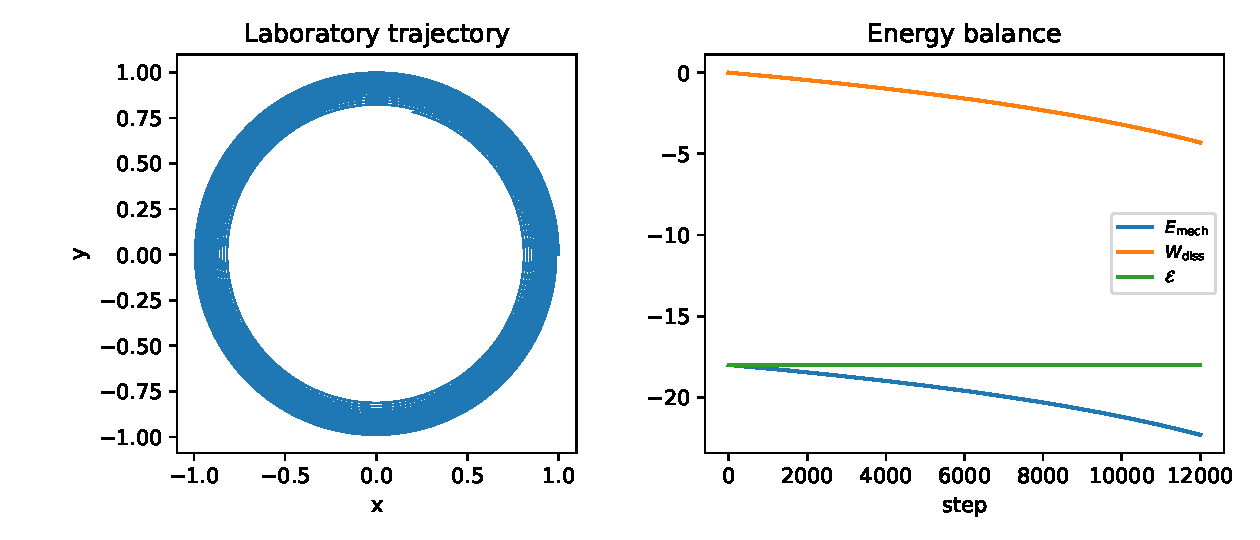
\includegraphics[width=0.92\linewidth]{figs/namcg_gr_simulation_corrected.pdf}
  \caption{Laboratory trajectory and energy balance for
    \eqref{eq:lab-ode} with the toy parameters
    \eqref{eq:toy-params}. The figure is a reduced model.}
  \label{fig:lab}
\end{figure}

If a previously generated PNG from the notes is used instead,
it belongs at this caption and nowhere else in the book.

\section{Code}
\label{sec:ch15-code}

The integrator lives in \texttt{code/namcg\_inspiral.py}. A
minimal version sufficient to produce Figure~\ref{fig:lab} is
the following.

\begin{lstlisting}[style=namcgPythonStyle, caption={Python implementation of the reduced inspiral laboratory velocity-Verlet integrator.}, label={lst:inspiral_code}]
import numpy as np
import matplotlib.pyplot as plt

def run_namcg_laboratory(
    G_toy=36.0,
    eta=0.006,
    M=1.0,
    mu=1.0,
    d0=1.0,
    dt=1.0e-3,
    num_steps=12000,
):
    r = np.array([d0, 0.0])
    v = np.array([0.0, np.sqrt(G_toy * M / d0)])
    traj = np.zeros((num_steps + 1, 2))
    E_mech = np.zeros(num_steps + 1)
    W_diss = np.zeros(num_steps + 1)
    traj[0] = r

    def a_N(r):
        d = np.linalg.norm(r)
        return -G_toy * M * r / d**3

    def a_d(r, v):
        d = np.linalg.norm(r)
        return -eta * v / d**4

    def mechanical_energy(r, v):
        d = np.linalg.norm(r)
        return 0.5 * mu * np.dot(v, v) - G_toy * M * mu / d

    E_mech[0] = mechanical_energy(r, v)
    for n in range(num_steps):
        F_d = mu * a_d(r, v)
        W_diss[n + 1] = W_diss[n] + np.dot(F_d, v) * dt
        v_half = v + 0.5 * dt * (a_N(r) + a_d(r, v))
        r = r + dt * v_half
        v = v_half + 0.5 * dt * (a_N(r) + a_d(r, v_half))
        traj[n + 1] = r
        E_mech[n + 1] = mechanical_energy(r, v)
    return traj, E_mech, W_diss

def plot_laboratory(traj, E_mech, W_diss, filename):
    E_bal = E_mech - W_diss
    fig, axes = plt.subplots(1, 2, figsize=(8.4, 3.6))
    axes[0].plot(traj[:, 0], traj[:, 1], lw=0.8)
    axes[0].set_aspect("equal")
    axes[0].set_xlabel("x")
    axes[0].set_ylabel("y")
    axes[0].set_title("Laboratory trajectory")
    t = np.arange(len(E_mech))
    axes[1].plot(t, E_mech, label=r"$E_{\mathrm{mech}}$")
    axes[1].plot(t, W_diss, label=r"$W_{\mathrm{diss}}$")
    axes[1].plot(t, E_bal, label=r"$\mathcal{E}$")
    axes[1].set_xlabel("step")
    axes[1].set_title("Energy balance")
    axes[1].legend(fontsize=8)
    fig.tight_layout()
    fig.savefig(filename)
    plt.close(fig)

if __name__ == "__main__":
    traj, E_mech, W_diss = run_namcg_laboratory()
    plot_laboratory(
        traj, E_mech, W_diss,
        "figs/namcg_gr_simulation_corrected.pdf",
    )
\end{lstlisting}

Run the file from the project root after creating \texttt{figs/}.
The script writes a vector PDF suitable for the print interior.
A PNG of the same figure, if already produced by an earlier
notebook, may be kept for draft viewing but should not be the
print original.

\section{How to misread the figure, and how not to}
\label{sec:ch15-misread}

The shrinking orbit is not a measurement of \(\eta\) in nature.
The value \(0.006\) was chosen so that decay is visible in
\(1.2\times 10^{4}\) steps. A realistic mutual-information tail
would produce a far smaller \(\eta\) at \(d\gg\ell_A+\ell_B\).

The flatness of \(\mathcal{E}(t)\) is not a proof of
Theorem~\ref{thm:conservation}. It is a check that the laboratory
implements the balance that the theorem requires of any legal
reduction. If \(\mathcal{E}\) is flat and the force law is not
\eqref{eq:Fdiss}, the check has been passed for the wrong theory.

Comparing the laboratory decay time with a LIGO inspiral time is
not a test of NAMCG. The laboratory has no gravitational waves,
no horizons, and no relativity. Section~\ref{sec:ch14-quad}
already stated the regime in which quadrupole losses dominate.

\section{Exercises}
\label{sec:ch15-exercises}

\begin{enumerate}
  \item \textbf{Zero drag.}
    Set \(\eta=0\) and confirm that \(E_{\mathrm{mech}}\) and
    \(|\mathbf{L}|\) are constant at the level of Verlet error.
    What is the size of that error as a function of \(\Delta t\)?
  \item \textbf{Balance.}
    With \(\eta=0.006\), plot \(\mathcal{E}(t)\) for
    \(\Delta t\in\{10^{-3},5\times 10^{-4},2\times 10^{-3}\}\).
    Does the drift shrink with \(\Delta t\)?
  \item \textbf{Illegal drag.}
    Replace \(d^{-4}\) by a constant \(\gamma\) and rerun. Track
    \(W_{\mathrm{diss}}\) as \(d\) decreases. Why is the late
    behaviour a counterexample to Exercise~5 of Chapter~14?
  \item \textbf{Angular momentum.}
    The drag~\eqref{eq:Fdiss} is antiparallel to \(\mathbf{v}\).
    Show that it exerts a torque and compute
    \(\mathrm{d}\mathbf{L}/\mathrm{d}t\). Confirm the identity
    on the numerical trajectory.
  \item \textbf{Units.}
    Restore SI symbols in~\eqref{eq:lab-ode} and assign dimensions
    to \(\eta\). What combination of \(\ell_A,\ell_B,c\) could
    supply those dimensions if \(\eta\) is built from
    \eqref{eq:I-tail}?
\end{enumerate}

\section{Bridge to Chapter~16}
\label{sec:ch15-bridge}

Every extra structure used in applications now has a name:
the regular core~\eqref{eq:f-reg}, the baryon-tracking extra
density of Assumption~\ref{ass:track}, the working drag of
Assumption~\ref{ass:drag}, and the laboratory of this chapter.
Chapter~16 collects the full list of assumptions from
Chapters~3--15, restates the derivation chain of Chapter~1 as a
single page, and writes the observations that would kill the
framework rather than merely constrain \(\eta\).